% === Cours de Java
% === Chapitre : Introduction
\section{D�velopper en \sigle{Java}}
\leconwithtoc

\subsection{La machine virtuelle}

\begin{frame}{Le probl�me de la portabilit�}
Il est difficile de d�velopper un programme \textit{multi-OS}
  \begin{itemize}
  \item Parties de code diff�rentes d'un OS � l'autre
  \item $\Longrightarrow$ ne tourne que sur un OS
  \end{itemize} 
\medskip
Intenable pour \sigle{Java} (\emph{applets})
  \begin{itemize}
  \item N�cessit� de developper un code \emph{portable}
  \end{itemize}
\medskip
R�ponse de \sigle{SUN} : la machine \emph{virtuelle} (JVM)
  \begin{itemize}
  \item Programmes \sigle{Java} d�velopp�s pour la JVM
  \item Comment les faire tourner sur une machine r�elle ?
  \end{itemize}
\end{frame}

\begin{frame}{La machine virtuelle}
Via un programme qui \emph{�mule} la \emph{machine virtuelle \sigle{Java}} (\sigle{JVM})  
\medskip
\begin{center}
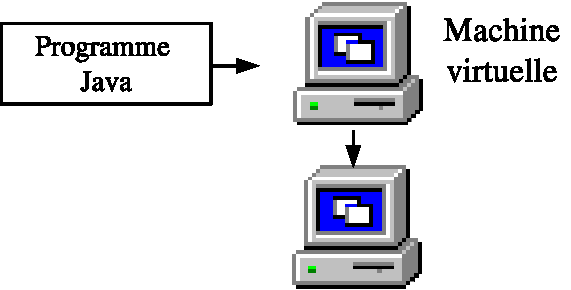
\includegraphics[scale=.8]{../img/java-jvm-jvm1} 
\end{center} 
\end{frame}

\begin{frame}{La machine virtuelle}
\sigle{Java} serait lent � interpr�ter (langage de haut niveau)
\begin{itemize}
\item Introduction d'un niveau interm�diaire : le \emph{\sigle{Bytecode}}
  \begin{itemize}
  \item Proche d'un langage d'assemblage
  \item Plus rapide � interpr�ter
  \item C'est en fait le langage de la \sigle{JVM} 
  \end{itemize}
\item \sigle{Java} est d'abord compil� en \sigle{Bytecode}
\end{itemize}
\bigskip
$\Longrightarrow$ \emph{Approche mixte} compilation/interpr�tation
\end{frame}

\begin{frame}{La machine virtuelle}
\begin{center}
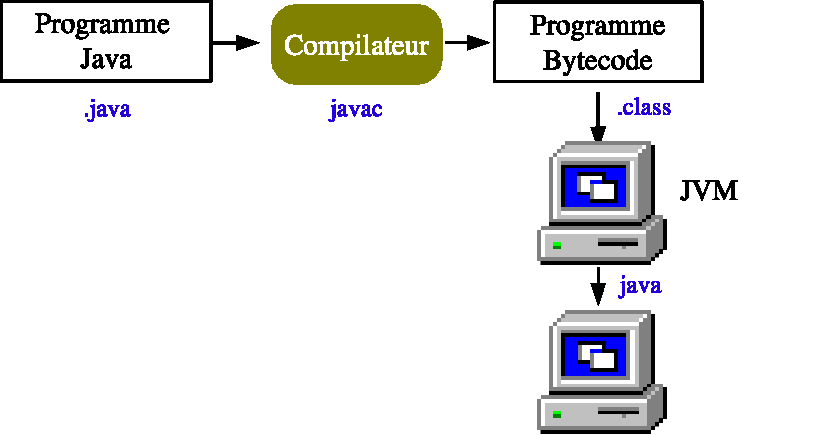
\includegraphics[scale=0.8]{../img/java-jvm-jvm2} 
\end{center}
\end{frame}

\begin{frame}[fragile]{Exemple: premier programme}
Prenons un exemple \textit{(fichier \code{Hello.java})}
\begin{Java}
// Mon premier programme
public class Hello {
  public static void main(String[] args) {
    System.out.println("Bonjour !");
  }
}
\end{Java}
\raisebox{2ex}{Compilons-le}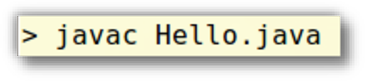
\includegraphics[scale=.8]{../img/javac} \raisebox{2ex}{\scriptsize(extrait d'une console)}\\
On obtient la version compil�e (\code|Hello.class|)\\
\raisebox{3ex}{Ex�cutons-la sur la machine virtuelle}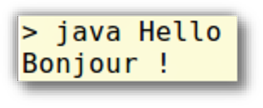
\includegraphics[scale=.8]{../img/java}
\end{frame}

\subsection{Les outils de d�veloppement}

\begin{frame}{Les outils de d�veloppement}
\emph{\sigle{JRE}} : \textit{Java Runtime Environment}
\begin{itemize}
\item Ce qui est n�cessaire � l'ex�cution
\item Accompagne les navigateurs \sigle{Web} par ex.
\end{itemize}
\bigskip
\emph{\sigle{JDK SE}} : \textit{Java Development Kit} (standard edition)
\begin{itemize}
\item Permet de developper en Java
  \begin{itemize}
  \item \emph{\sigle{javac}} : compilateur \sigle{Java} vers \sigle{bytecode}
  \item \emph{\sigle{java}} : la machine virtuelle \sigle{Java} 
  \item \emph{\sigle{javadoc}} : production automatique de documentation
  \item \dots
  \end{itemize}  
\item Gratuit, fourni par \sout{\sigle{SUN}} \sigle{Oracle}
\end{itemize}
\end{frame}

\begin{frame}{Les outils de d�veloppement}
Les \textit{\emph{E}nvironnement de \emph{D}�veloppement \emph{I}nt�gr�} : 
\emph{\sigle{Netbeans}}, \emph{\sigle{Eclipse}}, \dots
\begin{itemize}
\item Gratuits
\item Avantages
  \begin{itemize}
  \item �diteur, compilateur, d�buggeur et aide int�gr�s dans un m�me outil
  \item G�n�ration automatis�e de code 
  \end{itemize}
\item Inconv�nient : on maitrise moins tout le processus (quand �a ne marche pas, on ne comprend pas pourquoi !)
\end{itemize}
\end{frame}

\begin{frame}{Les outils de d�veloppement}
Autre possibilit� : les techniques brutes
\begin{itemize}
\item Un \emph{�diteur avec coloration syntaxique}
\item Gestion manuelle des noms et emplacements des fichiers
\item Compilation et ex�cution en ligne de commande
\end{itemize}
\bigskip
\begin{center}
\textit{Approche choisie � l'�cole pour vous faire \\comprendre ce qu'il y a derri�re}
\end{center}
\end{frame}

